\documentclass{article}
\usepackage{minted}
\usepackage[spanish]{babel}
\usepackage{hyperref}
\usepackage{graphicx}
\usepackage{xcolor}
\definecolor{LightGray}{gray}{0.85}
\graphicspath{ {./images/} }

%%%%%%%%%%%%%%%%%%%%%%%%%%%%%%%%%%%%%%%%%%%%%%%%%%%%%%
% COMIENZA EL DOCUMENTO
%%%%%%%%%%%%%%%%%%%%%%%%%%%%%%%%%%%%%%%%%%%%%%%%%%%%%%

\begin{document}

\tableofcontents
\newpage

\section{Configuración del fichero net.conf}
\begin{minted}
  [
    frame=lines,
    framesep=2mm,
    baselinestretch=1.2,
    bgcolor=LightGray,
    fontsize=\footnotesize
  ]{bash}
  redes@RED:~$ (nano|vim.tiny) net.conf # Tu editor favorito dentro de la VM
  # NO deben repetirse las umlX.Y o de lo contrario,
  # dará un error al lanzar el escenario
  defsw br12 uml1.0 uml2.0 # configura la conexión entre dos interfaces
  defsw net1 uml1.1 # configura la conexión para una sola interfaz
  defsw br345 uml3.0 uml4.1 uml5.2 # configura la conexión para tres interfaces
\end{minted}

\section{Preparación del entorno}
\begin{minted}
  [
    frame=lines,
    framesep=2mm,
    baselinestretch=1.2,
    bgcolor=LightGray,
    fontsize=\footnotesize
  ]{bash}
  # borra las configuraciones previamente existentes
  redes@RED:~$ sudo ifovsdel
  # configura las interfaces para lanzar el entorno
  redes@RED:~$ sudo ifovsparse net.conf
  # crea un rango de directorios desde uml1 a umlN
  redes@RED:~$ mkdir uml{1..N}
  # crea las uml declaradas anteriormente
  redes@RED:~$ lanza {1..N}
\end{minted}

\section{Finalización del entorno}
\begin{minted}
  [
    frame=lines,
    framesep=2mm,
    baselinestretch=1.2,
    bgcolor=LightGray,
    fontsize=\footnotesize
  ]{bash}
  # Ejecuta un ctrl+alt+del en cada una de las UML (forma suave de matar las UML)
  redes@RED:~$ for i in {1..N} ; do uml\_mconsole uml$i cad; done
  # Mata todos los subprocesos linux de golpe (forma dura de matar las UML)
  # Es el último recurso a utilizar en caso de que
  # el anterior comando no funcione
  redes@RED:~$ pkill linux
\end{minted}

\section{Iniciar sesión en una UML}
\begin{minted}
  [
    frame=lines,
    framesep=2mm,
    baselinestretch=1.2,
    bgcolor=LightGray,
    fontsize=\footnotesize
  ]{bash}
  uml1 login: root # entramos siempre como root
  root@uml1# # A partir de aqui, estamos dentro de una sesión bash en la UML1
\end{minted}

\section{Acceder al shell de Quagga}
\begin{minted}
  [
    frame=lines,
    framesep=2mm,
    baselinestretch=1.2,
    bgcolor=LightGray,
    fontsize=\footnotesize
  ]{bash}
  root@uml1# vtysh
  uml1# # Aqui ya estamos dentro de una sesión de Quagga
\end{minted}

\section{Acceder a la consola para introducir comandos de configuración}
\begin{minted}
  [
    frame=lines,
    framesep=2mm,
    baselinestretch=1.2,
    bgcolor=LightGray,
    fontsize=\footnotesize
  ]{lexer.py:IOSLexer -x}
  uml1# # Lo que está entre corchetes significa que es opcional
  uml1# conf[igure] term[inal]
  uml1(config)# ! Estamos dentro de la configuración de la UML
\end{minted}

\section{Acceder a una interfaz}
\begin{minted}
  [
    frame=lines,
    framesep=2mm,
    baselinestretch=1.2,
    bgcolor=LightGray,
    fontsize=\footnotesize
  ]{lexer.py:IOSLexer -x}
  uml1(config)# int[erface] eth0
  uml1(config-if)# # Estamos dentro de la interfaz eth0
\end{minted}

\section{Añadir una IP a la interfaz}
\begin{minted}
  [
    frame=lines,
    framesep=2mm,
    baselinestretch=1.2,
    bgcolor=LightGray,
    fontsize=\footnotesize
  ]{lexer.py:IOSLexer -x}
  uml1(config-if)# ip address 10.0.0.1/24
  uml1(config-if)# ipv6 address 2001:db8::50:10/64
  uml1(config-if)# no shutdown # IMPORTANTE para que la interfaz quede levantada
\end{minted}

\section{Activar retransmisión de paquetes}
\begin{minted}
  [
    frame=lines,
    framesep=2mm,
    baselinestretch=1.2,
    bgcolor=LightGray,
    fontsize=\footnotesize
  ]{lexer.py:IOSLexer -x}
  uml1(config)# # Lo que se le dice a la UML donde se ejecuta el siguiente
  uml1(config)# # comando es que actúe como router (encaminador)
  uml1(config)# ip[v6] forwarding
\end{minted}

\section{Anuncio de prefijo en IPv6}
\begin{minted}
  [
    frame=lines,
    framesep=2mm,
    baselinestretch=1.2,
    bgcolor=LightGray,
    fontsize=\footnotesize
  ]{lexer.py:IOSLexer -x}
  ! Los hosts a los que hayan que hacerles el anuncio del prefijo
  ! solo hay que hacerles un `no shutdown' en la interfaz asociada
  uml1(config-if)# ipv6 nd prefix 2001:db8:101:1::/64
  uml1(config-if)# no ipv6 nd suppress-ra
\end{minted}

\section{Guardar la configuración establecida}
\begin{minted}
  [
    frame=lines,
    framesep=2mm,
    baselinestretch=1.2,
    bgcolor=LightGray,
    fontsize=\footnotesize
  ]{lexer.py:IOSLexer -x}
  uml1(config)# write ! Guarda toda la configuración
\end{minted}

\section{Zebra}
\subsection{Interface Commands}
\subsubsection{Standard Commands}
\begin{minted}
  [
    frame=lines,
    framesep=2mm,
    baselinestretch=1.2,
    bgcolor=LightGray,
    fontsize=\footnotesize
  ]{lexer.py:IOSLexer -x}
  !!! Estos comandos es necesario estar dentro de la interfaz
  ! Apaga o levanta la interfaz
  [no] shutdown
  ! Añade una IP v4 o v6 a una interfaz
  [no] ip[v6] a[ddress] ADDRESS/PREFIX
\end{minted}

\subsection{Zebra Terminal Mode Commands}
\begin{minted}
  [
    frame=lines,
    framesep=2mm,
    baselinestretch=1.2,
    bgcolor=LightGray,
    fontsize=\footnotesize
  ]{lexer.py:IOSLexer -x}
  ! Muestra las rutas actuales que almacena zebra en su base de datos
  show ip[v6] route
  ! Muestra información sobre la interfaz
  show interface [INTERFACE] ! ej: eth0
\end{minted}

\section{RIP}
\subsection{Start RIPd}
\begin{minted}
  [
    frame=lines,
    framesep=2mm,
    baselinestretch=1.2,
    bgcolor=LightGray,
    fontsize=\footnotesize
  ]{bash}
  # Activar el demonio ripd en el fichero /etc/quagga/daemons
  ~$ systemctl restart quagga
  ~$ systemctl status quagga
\end{minted}

\subsection{Configuration}
\begin{minted}
  [
    frame=lines,
    framesep=2mm,
    baselinestretch=1.2,
    bgcolor=LightGray,
    fontsize=\footnotesize
  ]{lexer.py:IOSLexer -x}
  ! Habilita o deshabilita RIP
  [no] router rip
  ! Fija o no la interfaz RIP habilitada por ifname
  [no] network ifname ! ej.: network eth0
  ! Especifica o no un vecino RIP
  [no] neighbor a.b.c.d
  ! Controla split-horizon en la interfaz. Por defecto activado
  [no] ip split-horizon
\end{minted}

\subsection{Show RIP Information}
\begin{minted}
  [
    frame=lines,
    framesep=2mm,
    baselinestretch=1.2,
    bgcolor=LightGray,
    fontsize=\footnotesize
  ]{lexer.py:IOSLexer -x}
  ! Muestra rutas RIP
  show ip rip
  ! Muestra estado actual de RIP
  show ip rip status
\end{minted}

\section{RIPng}
\subsection{Start RIPngd}
\begin{minted}
  [
    frame=lines,
    framesep=2mm,
    baselinestretch=1.2,
    bgcolor=LightGray,
    fontsize=\footnotesize
  ]{bash}
  # Activar el demonio ripngd en el fichero /etc/quagga/daemons
  ~$ systemctl restart quagga
  ~$ systemctl status quagga
\end{minted}

\subsection{Configuration}
\begin{minted}
  [
    frame=lines,
    framesep=2mm,
    baselinestretch=1.2,
    bgcolor=LightGray,
    fontsize=\footnotesize
  ]{lexer.py:IOSLexer -x}
  ! Habilita o deshabilita RIPng
  [no] router ripng
  ! Fija o no la interfaz RIPng habilitada por ifname
  [no] network ifname ! ej.: network eth0
\end{minted}

\subsection{Show RIPng Information}
\begin{minted}
  [
    frame=lines,
    framesep=2mm,
    baselinestretch=1.2,
    bgcolor=LightGray,
    fontsize=\footnotesize
  ]{lexer.py:IOSLexer -x}
  ! Muestra rutas RIPng
  show ip ripng
\end{minted}

\section{OSPFv2}
\subsection{Configuration}
\begin{minted}
  [
    frame=lines,
    framesep=2mm,
    baselinestretch=1.2,
    bgcolor=LightGray,
    fontsize=\footnotesize
  ]{bash}
  # Activar el demonio ospfd en el fichero /etc/quagga/daemons
  ~$ systemctl restart quagga
  ~$ systemctl status quagga
\end{minted}

\subsection{Router}
\begin{minted}
  [
    frame=lines,
    framesep=2mm,
    baselinestretch=1.2,
    bgcolor=LightGray,
    fontsize=\footnotesize
  ]{lexer.py:IOSLexer -x}
  ! Activa o desactiva el proceso OSPF
  [no] router ospf
  ! Fija o quit el router-id del proceso OSPF
  [no] ospf router-id a.b.c.d
  ! Solo se anuncia la interfaz como link stub en router LSA
  ! Hay que ponerlo en las redes de usuario
  passive-interface ifname
  ! Habilita o deshabilita stub router advertisement support
  [no] max-metric router-lsa [on-startup|on-shutdown|administrative]
  ! Especifica o no las interfaces habilitadas en OSPF
  ! también puede ser en el formato a.b.c.d
  [no] network a.b.c.d/m area <0-4294967295>
\end{minted}

\subsection{Area}
\begin{minted}
  [
    frame=lines,
    framesep=2mm,
    baselinestretch=1.2,
    bgcolor=LightGray,
    fontsize=\footnotesize
  ]{lexer.py:IOSLexer -x}
  ! Agrega o desagrega rutas inter-área (solo válido para ABR)
  [no] area a.b.c.d range a.b.c.d/m ! Un ejemplo en la práctica de OSPFv2
  ! Define o elimina un área stub
  [no] area a.b.c.d sub [no-summary]
\end{minted}

\subsection{Showing OSPF Information}
\begin{minted}
  [
    frame=lines,
    framesep=2mm,
    baselinestretch=1.2,
    bgcolor=LightGray,
    fontsize=\footnotesize
  ]{lexer.py:IOSLexer -x}
  ! Muestra info de proposito general de OSPF
  show ip ospf
  ! Muestra estado y configuracion de la interfaz especifica OSPF (todas si
  ! no se especifica alguna)
  show ip ospf interface [INTERFACE]
  ! Muestra info de la BBDD OSPF
  show ip ospf database
  ! Muestra la tabla de rutas OSPF
  show ip ospf route
\end{minted}


\section{OSPFv3}
\subsection{Configuration}
\begin{minted}
  [
    frame=lines,
    framesep=2mm,
    baselinestretch=1.2,
    bgcolor=LightGray,
    fontsize=\footnotesize
  ]{bash}
  # Activar el demonio ospf6d en el fichero /etc/quagga/daemons
  ~$ systemctl restart quagga
  ~$ systemctl status quagga
\end{minted}

\subsection{Router}
\begin{minted}
  [
    frame=lines,
    framesep=2mm,
    baselinestretch=1.2,
    bgcolor=LightGray,
    fontsize=\footnotesize
  ]{lexer.py:IOSLexer -x}
  ! Acceder a la configuracion del router
  router ospf6
  ! Fijar un router-id
  router-id a.b.c.d ! ej: 0.0.0.1
  ! Bindea una interfaz a un area y comienza el envio de paquetes
  interface ifname area a.b.c.d ! ej: interface eth0 area 0.0.0.1
\end{minted}

\subsection{Interface}
\begin{minted}
  [
    frame=lines,
    framesep=2mm,
    baselinestretch=1.2,
    bgcolor=LightGray,
    fontsize=\footnotesize
  ]{lexer.py:IOSLexer -x}
  !!! Estos comandos es necesario estar dentro de la interfaz

  ! Establece coste de la interfaz. El valor por defecto depende
  ! del ancho de banda de la interfaz y del coste del ancho de
  ! banda de referencia
  ipv6 opsf6 cost COST ! ej: 2
  ! Establece coste del intervalo HELLO de la interfaz
  ipv6 opsf6 hello-interval HELLOINTERVAL ! ej: 60
  ! Establece intervalo Router Dead en la interfaz
  ipv6 ospf6 dead-interval DEADINTERVAL ! ej: 240
  ! Establece intervalo de retransmisión de la interfaz
  ipv6 ospf6 retransmit-interval RETRANSMITINTERVAL ! ej: 5
  ! Establece Router Priority de la interfaz
  ipv6 opsf6 priority PRIORITY ! ej: 5
  ! Establece Inf-Trans-Delay de la interfaz
  ipv6 ospf6 transmit-delay TRANSMITDELAY ! ej: 1
\end{minted}

\subsection{Showing OSPF Information}
\begin{minted}
  [
    frame=lines,
    framesep=2mm,
    baselinestretch=1.2,
    bgcolor=LightGray,
    fontsize=\footnotesize
  ]{lexer.py:IOSLexer -x}
  ! Muestra info acerca de OSPFv3 de la UML
  show ipv6 ospf6 [INSTANCE_ID]
  ! Muestra el resumen de la base de datos LSA
  show ipv6 ospf6 database
  ! Muestra la configuracion de la interfaz OSPF
  show ipv6 ospf6 interface
  ! Muestra el estado y el backup del vecino
  show ipv6 ospf6 neighbor
  ! Muestra la request-list del vecino
  show ipv6 ospf6 request-list A.B.C.D
  ! Muestra la tabla de rutas interna
  show ipv6 route ospf6
\end{minted}

\section{BGP}
\subsection{Start BGPd}
\begin{minted}
  [
    frame=lines,
    framesep=2mm,
    baselinestretch=1.2,
    bgcolor=LightGray,
    fontsize=\footnotesize
  ]{bash}
  # Activar el demonio bgpd en el fichero /etc/quagga/daemons
  ~$ systemctl restart quagga
  ~$ systemctl status quagga
\end{minted}

\subsection{BGP Router}
\begin{minted}
  [
    frame=lines,
    framesep=2mm,
    baselinestretch=1.2,
    bgcolor=LightGray,
    fontsize=\footnotesize
  ]{lexer.py:IOSLexer -x}
  ! [Des]habilita el proceso del protocolo BGP con el ASN especificado
  [no] router bgp asn ! ej: 65512
  ! Especifica el router-id (Identificador BGP)
  bgp router-id A.B.C.D ! ej: 10.0.0.1
\end{minted}

\subsection{BGP network}
\begin{minted}
  [
    frame=lines,
    framesep=2mm,
    baselinestretch=1.2,
    bgcolor=LightGray,
    fontsize=\footnotesize
  ]{lexer.py:IOSLexer -x}
  ! Añade/quita un anuncio BGP explícito
  [no] network A.B.C.D/M ! ej: 10.0.0.0/8
  ! Route aggregation
  !! Añade/quita un agregado de ruta
  [no] aggregate-address A.B.C.D/M ! ej: 192.168.0.0/16
\end{minted}

\subsection{Inyección de protocolos}
\begin{minted}
  [
    frame=lines,
    framesep=2mm,
    baselinestretch=1.2,
    bgcolor=LightGray,
    fontsize=\footnotesize
  ]{lexer.py:IOSLexer -x}
  ! Redistribuye RIP | OSPF al proceso BGP
  redistribute rip | ospf
\end{minted}

\subsection{Definición de vecinos}
\begin{minted}
  [
    frame=lines,
    framesep=2mm,
    baselinestretch=1.2,
    bgcolor=LightGray,
    fontsize=\footnotesize
  ]{lexer.py:IOSLexer -x}
  ! Crea/elimina un nuevo vecino cuyo ``remote-as'' es asn.
  ! peer puede ser una dirección IPv4 o IPv6
  [no] neighbor peer remote-as asn ! ej: neighbor 10.0.0.2 remote-as 65513
  ! Especifica la interfaz cuando el vecino está conectado por
  ! una dirección IPv6 de enlace local
  neighbor peer interface ifname ! ej: neighbor fe80::ff:fe00:1f0 interface eth0
\end{minted}

\newpage

\subsection{Filtrado de rutas}
  The \textbf{distribute-list} and \textbf{prefix-list} perform route filtering
  based on IP network addresses and netmasks of routes being advertised. The
  \textbf{distribute-list} refers to an ACL to match the individual networks and
  netmasks, while \textbf{prefix-list} refers to a prefix list to do this matching.
  In fact, the use of distribute-list and \textbf{prefix-list} for a particular
  BGP neighbor in a particular direction (in or out) is mutually exclusive,
  because they both accomplish the very same goal, just using a different
  route selection/filtering mechanism (an ACL vs. a prefix list).
  It is generally better to use prefix lists instead of ACLs - they are much
  more cleaner and more comprehensible, optimized to match networks/netmasks
  and subnets thereof.

  The \textbf{filter-list} performs route filtering based on the contents of the
  AS\_PATH attribute - the sequence and values of atonomous system numbers.
  To do this, you would configure an as-path ACL that contains one or more
  regular expressions matching the particular sequence of ASNs in the AS\_PATH
  attribute, and apply it to a neighbor and a particular direction with the
  \textbf{filter-list} command. With a \textbf{filter-list}, you do not perform
  route matching/filtering based on IP addresses and netmasks.

\begin{minted}
  [
    frame=lines,
    framesep=2mm,
    baselinestretch=1.2,
    bgcolor=LightGray,
    fontsize=\footnotesize
  ]{lexer.py:IOSLexer -x}
  ! Filtrado de prefijos
  ! ej: neighbor fe80::ff:fe00:1f0 prefix-list peer-out out
  neighbor peer prefix-list name [in|out]
  neighbor peer distribute-list name [in|out]
  ! ej: neighbor 10.0.0.1 route-map internal-rtm out
  neighbor peer route-map name [in|out]
\end{minted}

\subsection{AS\_PATH: Regex}
\begin{minted}
  [
    frame=lines,
    framesep=2mm,
    baselinestretch=1.2,
    bgcolor=LightGray,
    fontsize=\footnotesize
  ]{bash}
  . Cualquier carácter.
  * 0 o más apariciones del patrón.
  + 1 o más apariciones del patrón.
  ? 0 ó 1 apariciones del patrón.
  ^ Comienzo de línea.
  $ Final de línea.
  _ Concuerda con el espacio y la coma, así como con el
  delimitador de conjunto de ASN { y }, y con el delimitador
  de confederación ( y ). También concuerda con el principio
  y final de línea.
\end{minted}

\subsection{Muestra Rutas BGP por el AS\_PATH}
\begin{minted}
  [
    frame=lines,
    framesep=2mm,
    baselinestretch=1.2,
    bgcolor=LightGray,
    fontsize=\footnotesize
  ]{lexer.py:IOSLexer -x}
  ! muestra todas las rutas BGP que contienen el ASN 1180
  show ip bgp regexp _1180_
\end{minted}

\subsection{AS Path Access List}
\begin{minted}
  [
    frame=lines,
    framesep=2mm,
    baselinestretch=1.2,
    bgcolor=LightGray,
    fontsize=\footnotesize
  ]{lexer.py:IOSLexer -x}
  ! Define una nueva lista de acceso
  ip as-path access-list word {permit|deny} line
  ! Ejemplos con explicación
  ! n1 sólo permite rutas originadas en el AS100.
  ip as-path access-list n1 permit _100$
  ! n2 sólo permite rutas que pasen por AS102.
  ip as-path access-list n2 permit _102_
  ! n3 prohíbe todas las rutas que pasen (o provengan) de AS105.
  ip as-path access-list n3 deny _105_
  ip as-path access-list n3 permit .*
\end{minted}

\subsection{Verifica las rutas anunciadas por BGP}
\begin{minted}
  [
    frame=lines,
    framesep=2mm,
    baselinestretch=1.2,
    bgcolor=LightGray,
    fontsize=\footnotesize
  ]{lexer.py:IOSLexer -x}
  show ip bgp
\end{minted}

\section{Open VSwitch}

\begin{minted}
  [
    frame=lines,
    framesep=2mm,
    baselinestretch=1.2,
    bgcolor=LightGray,
    fontsize=\footnotesize
  ]{bash}
  # Crear un puente
  ovs-vsctl add-br <bridge>
  # Añadir un puerto a un bridge
  ovs-vsctl add-port <bridge> <port>
  # Listar bridges
  ovs-vsctl list-br
  # Listar puertos de un bridge
  ovs-vsctl list-ports <bridge>
  # Listar información de un puerto (o de todos)
  ovs-vsctl list port [<puerto>]
  # Mostrar información de un interfaz (o todos)
  ovs-vsctl list interface [<interface>]
  # Listar información de la base de datos
  ovs-vsctl list <table>
\end{minted}

\section{OpenFlow}

\subsection{Obtener número de puerto OpenFlow (útil para definir flujos)}

\begin{minted}
  [
    frame=lines,
    framesep=2mm,
    baselinestretch=1.2,
    bgcolor=LightGray,
    fontsize=\footnotesize
  ]
  {bash}
  redes@RED:~# ovs-vsctl add-port br0 \
  > uml1.0 -- set Interface uml1.0 ofport_request=1
  redes@RED:~# ovs-vsctl get Interface uml1.0 ofport
  1
  redes@RED:~# ovs-ofctl show br0
  1(uml1.0): addr      : 12:18:12:57:61:4f
            config     : 0
            state      : 0
            current    : 10MB-FD COPPER
            speed      : 10 Mbps now, 0 Mbps max
  2(uml2.0): addr      : 1e:22:97:0a:eb:f6
            config     : 0
            state      : 0
            current    : 10MB-FD COPPER
            speed      : 10 Mbps now, 0 Mbps max
  LOCAL(br0): addr     : 46:5a:3b:0a:b0:44
            config     : 0
            state      : 0
            speed      : 0 Mbps now, 0 Mbps max
\end{minted}

\subsection{Mostrar los flujos definidos actualmente}

\begin{minted}
  [
    frame=lines,
    framesep=2mm,
    baselinestretch=1.2,
    bgcolor=LightGray,
    fontsize=\footnotesize
  ]{bash}
  redes@RED:~# ovs-ofctl dump-flows br0
  NXST_FLOW reply (xid=0x4):
  cookie=0x0, duration=82.214s,
  table=0, n_packets=0, n_bytes=0, idle_age=82,
  priority=0 actions=NORMAL
  cookie=0x0, duration=5277.696s,
  table=0, n_packets=9649, n_bytes=945602, idle_age=0,
  priority=50,in_port=1 actions=resubmit(,101)
\end{minted}

\subsection{Añadir flujos}

\begin{minted}
  [
    frame=lines,
    framesep=2mm,
    baselinestretch=1.2,
    bgcolor=LightGray,
    fontsize=\footnotesize
  ]{bash}
  redes@RED:~# ovs-ofctl add-flow br0 \
  > "table=0, priority=210 \
  > ipv6_src=fe80::ff:fe00:1f0/128 icmp6 icmp_type=134 actions=normal"
  redes@RED:~# ovs-ofctl add-flow br0 \
  > "table=0, priority=200 \
  > icmp6 icmp_type=134 actions=drop"
  redes@RED:~# ovs-ofctl add-flow br0 \
  > "table=0, priority=100 dl_dst=01:00:00:00:00:00/01:00:00:00:00:00 \
  > actions=flood"
\end{minted}

\subsection{Borrar flujos}

\begin{minted}
  [
    frame=lines,
    framesep=2mm,
    baselinestretch=1.2,
    bgcolor=LightGray,
    fontsize=\footnotesize
  ]{bash}
  redes@RED:~# ovs-ofctl del-flows br0 \
  > "ipv6_src=fe80::ff:fe00:1f0/128 icmp6 icmp_type=134"
  redes@RED:~# ovs-ofctl del-flows br0
\end{minted}

% \newpage

\subsection{QoS}

\begin{figure}[h]
  \centering
  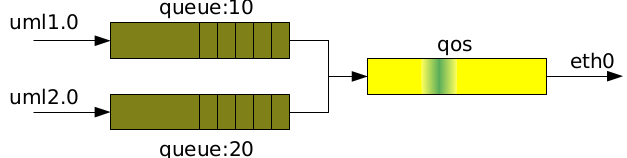
\includegraphics[width=10cm]{qos.png}
\end{figure}
\subsubsection{QoS. Definición de colas}

\begin{minted}
  [
    frame=lines,
    framesep=2mm,
    baselinestretch=1.2,
    bgcolor=LightGray,
    fontsize=\footnotesize
  ]
  {bash}
  redes@RED:~# ovs-vsctl -- \
  > add-br br0 -- \
  > add-port br0 eth0 -- \
  > add-port br0 uml1.0 -- set interface uml1.0 ofport_request=5 -- \
  > add-port br0 uml2.0 -- set interface uml2.0 ofport_request=6
  redes@RED:~# ovs-vsctl create queue other-config:max-rate=10000000
    8ad26ce4-ee2f-4fb1-949a-3ea41e8bb6ed
  redes@RED:~# ovs-vsctl create queue other-config:max-rate=20000000
    15e25965-db81-474d-b609-0a435b96bce1
  redes@RED:~# ovs-vsctl create qos type=linux-htb \
  > other-config:max-rate=1000000000 \
  > queues:10=8ad26ce4-ee2f-4fb1-949a-3ea41e8bb6ed \
  > queues:20=15e25965-db81-474d-b609-0a435b96bce1
  > 97ff4d44-de16-4ac9-8989-5c6ceff774c1
  redes@RED:~# ovs-vsctl set port eth0 qos=97ff4d44-de16-4ac9-8989-5c6ceff774c1
\end{minted}

\textbf{Alternativa}: Para no tener que anotar los ids de las colas, se puede
hacer todo en una sola orden:

\begin{minted}
  [
    frame=lines,
    framesep=2mm,
    baselinestretch=1.2,
    bgcolor=LightGray,
    fontsize=\footnotesize
  ]{bash}
  redes@RED:~# ovs-vsctl -- \
  > add-br br0 -- \
  > add-port br0 eth0 -- \
  > add-port br0 uml1.0 -- set interface uml1.0 ofport_request=5 -- \
  > add-port br0 uml2.0 -- set interface uml2.0 ofport_request=6 -- \
  > set port eth0 qos=@newqos -- \
  > --id=@newqos create qos type=linux-htb \
  > other-config:max-rate=1000000000 \
  > queues:10=@uml10queue \
  > queues:20=@uml20queue -- \
  > --id=@uml10queue create queue other-config:max-rate=10000000 -- \
  > --id=@uml20queue create queue other-config:max-rate=20000000
\end{minted}

\subsubsection{Listar colas}

\begin{minted}
  [
    frame=lines,
    framesep=2mm,
    baselinestretch=1.2,
    bgcolor=LightGray,
    fontsize=\footnotesize
  ]{bash}
  redes@RED:~# ovs-vsctl list queue
  _uuid: 8ad26ce4-ee2f-4fb1-949a-3ea41e8bb6ed
  dscp: []
  external_ids: {}
  other_config: {max-rate="10000000"}
  _uuid: 15e25965-db81-474d-b609-0a435b96bce1
  dscp: []
  external_ids: {}
  other_config: {max-rate="20000000"}
\end{minted}

\subsubsection{Definición de flujos para las colas creadas}

\begin{minted}
  [
    frame=lines,
    framesep=2mm,
    baselinestretch=1.2,
    bgcolor=LightGray,
    fontsize=\footnotesize
  ]{bash}
  redes@RED:~# ovs-vsctl list qos
  _uuid        : 97ff4d44-de16-4ac9-8989-5c6ceff774c1
  external_ids : {}
  other_config : {max-rate="10000000000"}
  queues       : {10=8ad26ce4-ee2f-4fb1-949a-3ea41e8bb6ed,
                  20=15e25965-db81-474d-b609-0a435b96bce1}
  type         : linux-htb
  redes@RED:~# ovs-ofctl add-flow br0 in_port=5,actions=set_queue:10,normal
  redes@RED:~# ovs-ofctl add-flow br0 in_port=6,actions=set_queue:20,normal
\end{minted}

\subsubsection{Cambio de los parámetros de una cola en tiempo real}
% TODO captura de este trozo de codigo
\begin{figure}[h]
  \centering
  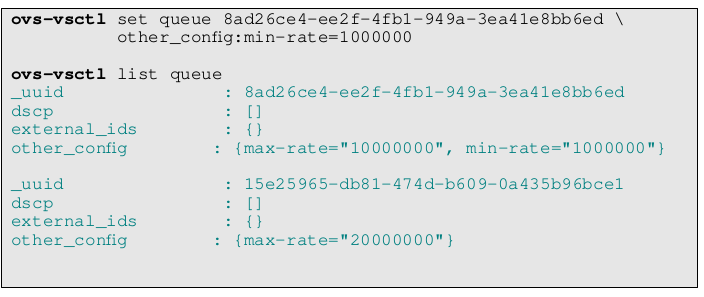
\includegraphics[width=10cm]{0_qos.png}
\end{figure}

\newpage

\subsubsection{Limitar el tráfico multicast por todos los enlaces}
% TODO captura de este trozo de codigo
\begin{figure}[h]
  \centering
  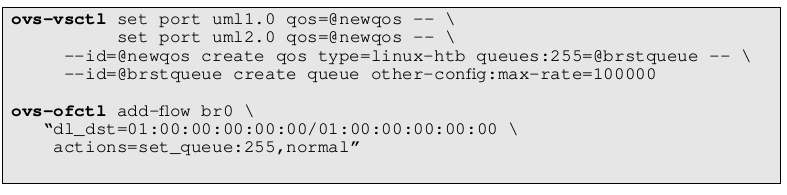
\includegraphics[width=10cm]{1_qos.png}
\end{figure}

\subsection{Mirroring}

\begin{figure}[h]
  \centering
  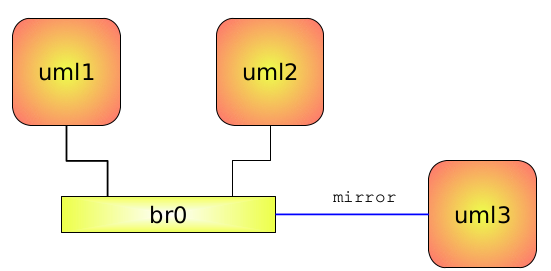
\includegraphics[width=10cm]{mirroring.png}
\end{figure}

\begin{minted}
  [
    frame=lines,
    framesep=2mm,
    baselinestretch=1.2,
    bgcolor=LightGray,
    fontsize=\footnotesize
  ]{bash}
  redes@RED:~# ovs-vsctl add-br br0
  redes@RED:~# ovs-vsctl add-port br0 uml1.0
  redes@RED:~# ovs-vsctl add-port br0 uml2.0
  redes@RED:~# ovs-vsctl add-port br0 uml3.0 -- \
  > --id=@p get port uml3.0 -- \
  > --id=@m create mirror name=m0 select-all=true output-port=@p -- \
  > set bridge br0 mirrors=@m
\end{minted}

\newpage

\subsubsection{Seleccionar solo un puerto}

\begin{minted}
  [
    frame=lines,
    framesep=2mm,
    baselinestretch=1.2,
    bgcolor=LightGray,
    fontsize=\footnotesize
  ]{bash}
  redes@RED:~# ovs-vsctl add-br br0
  redes@RED:~# ovs-vsctl add-port br0 uml1.0
  redes@RED:~# ovs-vsctl add-port br0 uml2.0
  redes@RED:~# ovs-vsctl add-port br0 uml3.0
  redes@RED:~# ovs-vsctl --id=@p1 get port uml1.0 -- \
  > --id=@p get port uml3.0 -- \
  > --id=@m create mirror name=m0 \
  > select_dst_port=@p1 select_src_port=@p1 output-port=@p -- \
  > set bridge br0 mirrors=@m
\end{minted}

\subsection{MPLS}

\subsubsection{MPLS. Añadir etiqueta MPLS}
% TODO meter imagen MPLS 1
\begin{figure}[h]
  \centering
  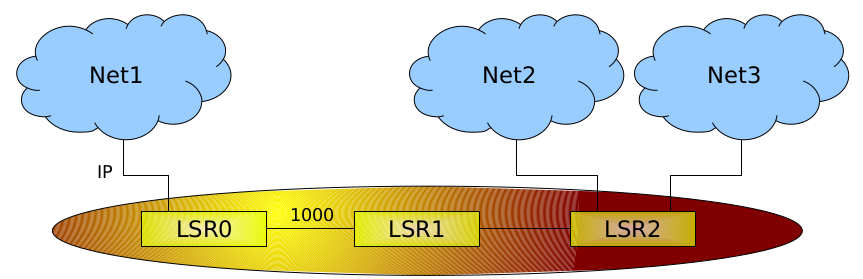
\includegraphics[width=10cm]{1_add_mpls.png}
\end{figure}

\textbf{IMPORTANTE}: Es necesario especificar el tipo Ethernet
de MPLS: 0x8847 para MPLS unicast y 0x8848 para multicast

\begin{minted}
  [
    frame=lines,
    framesep=2mm,
    baselinestretch=1.2,
    bgcolor=LightGray,
    fontsize=\footnotesize
  ]{bash}
  redes@RED:~# ovs-ofctl add-flow LSR0 'in_port=1, ip, nw_dst=192.168.0.0/16,
  > actions=push_mpls:0x8847,set_field:1000->mpls_label, output:2'
\end{minted}

\subsubsection{MPLS. Modificar etiqueta MPLS}
% TODO meter imagen MPLS 2
\begin{figure}[h]
  \centering
  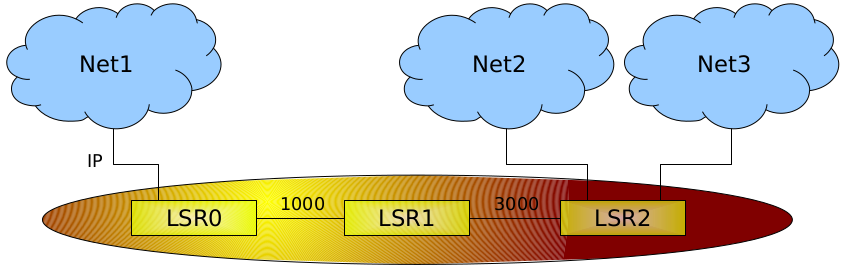
\includegraphics[width=10cm]{2_edit_mpls.png}
\end{figure}
\begin{minted}
  [
    frame=lines,
    framesep=2mm,
    baselinestretch=1.2,
    bgcolor=LightGray,
    fontsize=\footnotesize
  ]{bash}
  redes@RED:~# ovs-ofctl add-flow LSR1 'in_port=1, mpls, mpls_label=1000,
  > actions=set_field:3000->mpls_label, output:2'
\end{minted}

\subsubsection{MPLS. Eliminar etiqueta MPLS}
% TODO meter imagen MPLS 3
\begin{figure}[h]
  \centering
  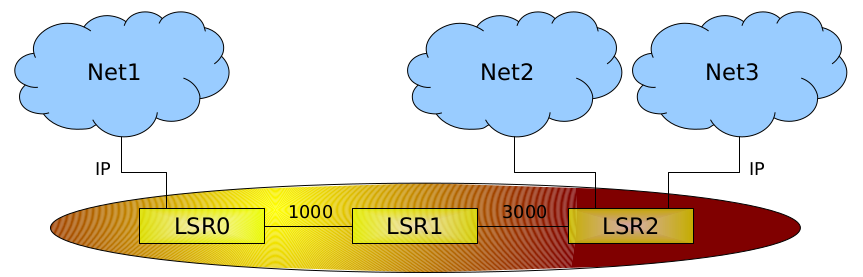
\includegraphics[width=10cm]{3_delete_mpls.png}
\end{figure}
\begin{minted}
  [
    frame=lines,
    framesep=2mm,
    baselinestretch=1.2,
    bgcolor=LightGray,
    fontsize=\footnotesize
  ]{bash}
  redes@RED:~# ovs-ofctl add-flow LSR2 'in_port=1, mpls,
  > mpls_label=3000, actions=pop_mpls:0x0800, output:3'
\end{minted}

\section{Configurar los demonios de Quagga}
\begin{minted}
  [
    frame=lines,
    framesep=2mm,
    baselinestretch=1.2,
    bgcolor=LightGray,
    fontsize=\footnotesize
  ]{bash}
  root@uml1# (nano|vim.tiny) /etc/quagga/daemons # Accedemos a los demonios de Quagga
\end{minted}

\section{Reiniciar y comprobar los demonios activos de Quagga}
\begin{minted}
  [
    frame=lines,
    framesep=2mm,
    baselinestretch=1.2,
    bgcolor=LightGray,
    fontsize=\footnotesize
  ]{bash}
  root@uml1# systemctl restart quagga
  root@uml1# systemctl status quagga
\end{minted}

\section{Atajos útiles de líneas de comandos}
\begin{itemize}
  \item Ctrl+a: Ir al inicio de la línea
  \item Ctrl+e: Ir al final de la línea
  \item Ctrl+w: Borra la palabra que está delante del cursor
  \item Ctrl+d: borra el caracter delante del cursor (supr de toda la vida)
  \item Ctrl+\_: Deshace el último cambio (El Ctrl+z de toda la vida)
  \item Ctrl+r: Busca por el historial del shell hacia atrás
  \item Ctrl+p: Como la flecha hacia arriba
  \item Ctrl+n: Como la flecha hacia abajo
  \item Ctrl+b: Como la flecha hacia la izquierda
  \item Ctrl+f: Como la flecha hacia la derecha
\end{itemize}

\end{document}

